\section{Algoritmi}\label{algoritmi}

\subsection{Notazione}\label{notazione}

La notazione utilizzata è la seguente:

\begin{itemize}
    \item \textit{user}: l'utente
    \item \textit{item}: l'oggetto
    \item \textit{rating}: valutazione/i
    \item $R$ : l'insieme di tutti i \textit{rating}.
    \item $R_{train}$, $R_{test}$ e $\hat{R}$ indicano il set di addestramento, il set di test e l'insieme dei \textit{rating} previsti.
    \item $U$ : l'insieme di tutti gli \textit{user}. $u$ e $v$ indicano gli \textit{user}.
    \item $I$ : l'insieme di tutti gli \textit{item}. $i$ e $j$ indicano gli \textit{item}.
    \item $U_i$ : l'insieme di tutti gli \textit{user} che hanno valutato l'\textit{item} $i$.
    \item $U_{ij}$ : l'insieme di tutti gli \textit{user} che hanno valutato sia l'\textit{item} $i$ che l'\textit{item} $j$.
    \item $I_u$ : l'insieme di tutti gli \textit{item} valutati dallo \textit{user} $u$.
    \item $I_{uv}$ : l'insieme di tutti gli \textit{item} valutati sia dallo \textit{user} $u$ che dallo \textit{user} $v$.
    \item $r_{ui}$ : il \textit{rating} \textit{vero} dello \textit{user} $u$ per l'\textit{item} $i$.
    \item $\hat{r}_{ui}$ : il \textit{rating} \textit{stimato} dello \textit{user} $u$ per l'\textit{item} $i$.
    \item $b_{ui}$ : il \textit{rating} di base dello \textit{user} $u$ per l'\textit{item} $i$.
    \item $\mu$ : la media di tutti i \textit{rating}.
    \item $\mu_u$ : la media di tutti i \textit{rating} dati dallo \textit{user} $u$.
    \item $\mu_i$ : la media di tutti i \textit{rating} date all'\textit{item} $i$.
    \item $\sigma_u$ : la deviazione standard di tutti i \textit{rating} dati dallo \textit{user} $u$.
    \item $\sigma_i$ : la deviazione standard di tutte le valutazioni date all'\textit{item} $i$.
    \item $N_i^k(u)$ : i $k$ vicini più prossimi dello \textit{user} $u$ che hanno valutato l'\textit{item} $i$. Questo insieme è calcolato utilizzando una metrica di similarità.
    \item $N_u^k(i)$ : i $k$ vicini più prossimi dell'\textit{item} $i$ che sono valutati dallo \textit{user} $u$. Questo insieme è calcolato utilizzando una metrica di similarità.
\end{itemize}


\subsection{Algoritmi per Feedback Esplicito}\label{algoritmi-per-feedback-esplicito}

\subsubsection{Matrix Factorization}\label{matrix-factorization}

\subsubsection{KNN}\label{knn}

\subsubsection{CoClustering}\label{coclustering}

\subsubsection{Slope One}\label{slopeone}

L'algoritmo Slope One, introdotto da Daniel Lemire e Anna Maclachlan\cite{SlopeOne}, è una delle soluzioni più semplici ed efficienti di collaborative filtering.
%
Le caratteristiche che lo rendono un ottimo algoritmo per la recommendation sono:
\begin{itemize}
    \item la semplicità e facilità di implementazione
    \item velocità di calcolo: come verrà presentato più avanti alcuni valori calcolati possono essere salvati e aggiornati all'occorrenza rendendo il calcolo molto più veloce
    \item scalabilità: l'algoritmo può essere abbastanza efficace su dataset di dimensioni moderate, soprattutto se si utilizzano tecniche di compressione dei dati
    \item facilità di interpretazione
\end{itemize}
%
Viene proposto un predittore basato su differenze di \textit{rating} lineari che ha un'efficienza $O(nm)$ per predizione e $O(mn^2)$ per addestramento, dove:

\begin{itemize}
    \item $m$ = numero di \textit{user}
    \item $n$ = numero di \textit{item}
\end{itemize}

L'algoritmo si basa sulla differenza media tra le valutazioni di due \textit{item} per predire il \textit{rating} mancante. La differenza media dei \textit{rating} di due \textit{item} $i$ e $j$ viene calcolata come:

\[
    \text{dev}(i, j) = \frac{1}{|U_{i,j}|} \sum\limits_{u \in U_{i,j}} (r_{u,i} - r_{u,j})
\]

La matrice simmetrica definita da $\text{dev}(i, j)$ può essere computata una volta e aggiornata velocemente quando vengono aggiunti nuovi dati.

La predizione viene dunque calcolata come:

\[
    \hat{r}_{ui} = \mu_u + \frac{1}{|R_i(u)|} \sum\limits_{j \in R_i(u)} \text{dev}(i, j)
\]

dove:

\begin{itemize}
    \item $R_j = \{ i \mid i \in S(u), i \neq j, |S_{j,i}(\chi)| > 0 \}$ è l'insieme degli \textit{item} rilevanti
    \item $S(u)$ è il sottoinsieme degli item valutati dallo \textit{user} $u$
    \item $S_{j,i}(\chi)$ è l'insieme di tutte le valutazioni $u$ nel dataset $\chi$ che contengono gli \textit{item} $i$ e $j$
\end{itemize}

\begin{figure}[H]
    \centering
    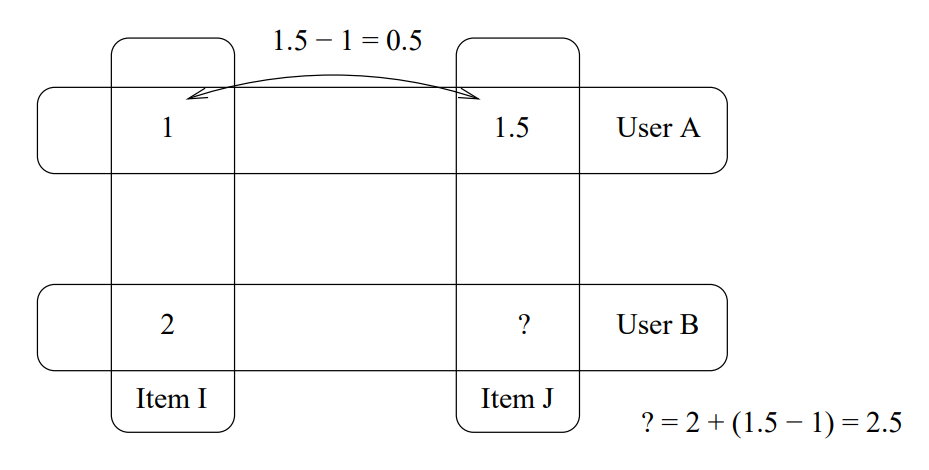
\includegraphics[keepaspectratio]{figures/algorithms/slope_one.PNG}
    \caption{Base dello schema Slope One: le valutazioni dello \textit{user} A di due \textit{item} e la valutazione  dello \textit{user} B di un \textit{item} comune vengono utilizzate per prevedere la valutazione sconosciuta dello \textit{user}.}
    \label{fig:slopeone}
\end{figure}

L'algoritmo soffre di diverse problematiche:
\begin{itemize}
    \item sparsità dei dati: le formule presentate prima sono approssimate considerando un dataset non sparso. Nel caso di matrici molto sparse l'algoritmo non sarà in grado di fare previsioni accurate
    \item scalabilità limitata su dataset molto grandi: la memoria necessaria per memorizzare le differenze medie dei \textit{rating} può aumentare rapidamente
    \item non tiene conto nè di personalizzazioni per \textit{user} 
    \item difficoltà a gestire grandi variazioni nelle valutazioni degli utenti
\end{itemize}

L'approccio può essere esteso a modelli ponderati e versioni più avanzate, come per esempio \emph{Weighted Slope One}, che pesa le differenze di \textit{rating} in base alla frequenza di coppie di \textit{item} valutati, e \emph{Regression-based Slope One}, che introduce funzioni non lineari per migliorare la precisione delle previsioni.


\subsubsection{Evaluation esplicita}\label{evaluation-esplicita}

\subsubsection{Algoritmi per Feedback Implicito}\label{algoritmi-per-feedback-implicito}

\subsubsection{ALS (Alternating Least Squares)}\label{als-alternating-least-squares}

\subsubsection{BPR (Bayesian Personalized Ranking)}\label{bpr-bayesian-personalized-ranking}

\subsubsection{LMF (Logistic Matrix Factorization)}\label{lmf-logistic-matrix-factorization}

\subsubsection{Evaluation implicita}\label{evaluation-implicita}

\subsubsection{Algoritmi per la Similarità Item-Item}\label{algoritmi-per-la-similarita-item-item}

\subsubsection{Algoritmi Ibridi}\label{algoritmi-ibridi}

\subsubsection{LightFM}\label{lightfm}

\subsubsection{Introduzione a Modelli di Deep Learning}\label{introduzione-a-modelli-di-deep-learning}
